\chapter{Background}
\label{chap:Background}
In this chapter, we provide background knowledge about Smartwatches and Bluetooth as well as Random Forest and Evaluation metrics.


\section{Smartwatches}
\label{sec:smartwatches}
There exist many brands of smartwatches running multiple operating systems. \textit{WearOS}, \textit{WatchOS} and \textit{Tizen} are amongst the main actors. WatchOS and Tizen are dedicated to run principally on Apple Watch and Samsung watches respectively; whereas WearOS is run by many different brand such as Huawei, Fossil, Motorola or even Louis Vuitton. In this thesis, we focus on three different smartwatch brands: \textbf{Huawei}, \textbf{Fossil} and \textbf{Apple}, which represents more than 40\% of the market share as of 2019. Fig.~\ref{fig:marketshare smartwatches.jpg} shows the market share of smartwatches by brands.


\begin{figure}[H]
 \centering
 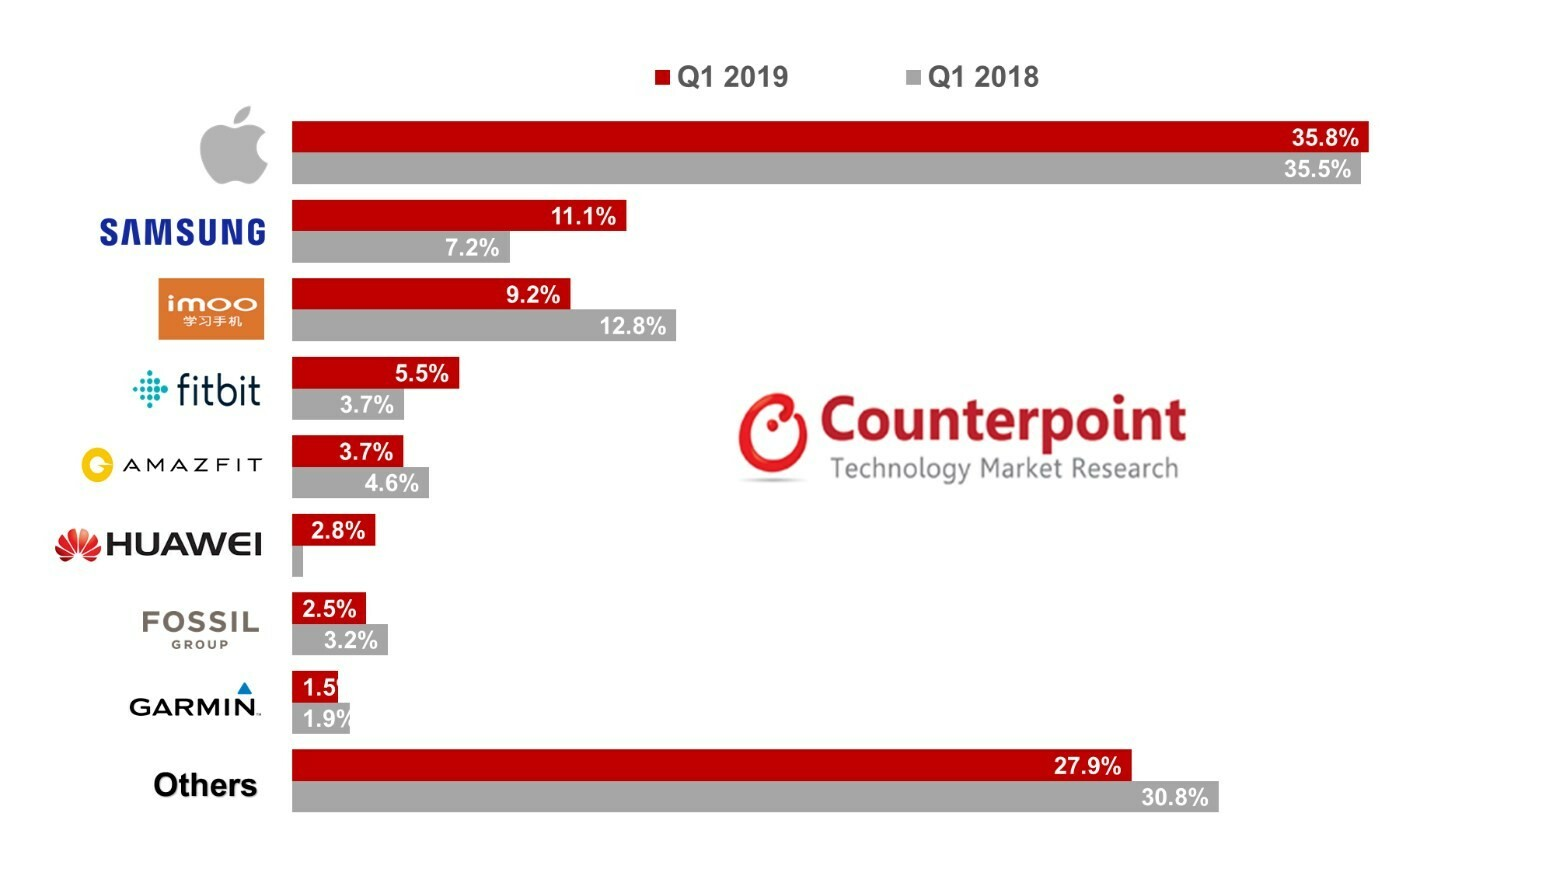
\includegraphics[width=0.9\textwidth]{figures/marketshare smartwatches.jpg}
 \caption[test]{Market share of smartwatches by brand in 2018 and 2019.\footnotemark}
 \label{fig:marketshare smartwatches.jpg}
\end{figure}
\footnotetext{Picture taken from https://www.notebookcheck.net/Latest-report-shows-1-in-every-3-smartwatches-sold-in-2019-so-far-was-an-Apple-Watch.420045.0.html}




\paragraph{Connectivity.} Most smartwatches are equipped with both Wi-Fi and Bluetooth interfaces. Even though Wi-Fi is supposed to provide a better throughput to access the Internet, a study shows that Bluetooth traffic is responsible for more than 91\% of the total traffic~\cite{10.1145/3081333.3081351}. The main reason is to save energy, since Bluetooth consumes less than Wi-Fi. Many possible events can be at the origin of data transfer over Bluetooth: push notifications\footnote{\textbf{Push notifications} are piece of information possibly coming from the outside world to notify the user of a particular event}, background updates or more naturally the user's interaction with the smartwatch.

\paragraph{Application Store.} Most smartwatches allow anyone to develop and deploy applications on their application store. However, it has to be noted that application stores of smartwatches are much more constrained than smartphone's application stores. In fact, smartwatches stores are more focused on Health, Fitness and Reminders applications; games for instance are almost non-existent due to the small screen size of smartwatches. 


\section{Bluetooth}
\label{sec:Bluetooth}
Bluetooth is a full stack protocol which is widely used to create Wireless Personal Area Network (WPAN). Nowadays, most personal mobile devices are equipped with Bluetooth interfaces. In that manner, the Bluetooth Special Interest Group (SIG) reported an expected increase from 0.9 billion annual unit shipment in 2020 to 1.5 billion in 2024 for data transfer devices such as smartwatches \cite{bluetoothMarket}. In this section we explain only relevant background about Bluetooth and we refer the reader to the Bluetooth Core specifications for further technical details \cite{bluetoothSpecs}.



\paragraph{Bluetooth Classic and Low Energy.} Two types of Bluetooth operate: Bluetooth Classic (Also known as BR/EDR) and Bluetooth Low Energy (BLE). Bluetooth Classic is intended for communication with intensive data transfer, while BLE aims to provide a communication that is energy efficient. Since most smartwatches are using Bluetooth Classic only, we will simply use Bluetooth to refer to Bluetooth Classic. 


\paragraph{Frequency-Hopping Spread Spectrum.} Bluetooth uses frequency-hopping spread spectrum (FHSS). It consists of dividing the allocated spectrum into narrow band subchannels and the time into slots of 625ns duration. In each time slot, a designated frequency band is used to transmit the signal. The frequency-hopping sequence is pseudo randomly generated and is derived by the peers taking part in the communication before the actual data transfer begins. When Bluetooth senses too much interference on a particular frequency band, it performs adaptive hopping which will bane the usage of this band of a period of time.  


\paragraph{Eavesdropping Bluetooth traffic.} Because of the FHSS scheme, it has long been considered technically difficult to eavesdrop Bluetooth communications. However, due to hardware improvements, many devices with Bluetooth eavesdropping capabilities start emerging. The cost and the efficiency of these devices vary a lot. Devices such as Ellisys Vanguard\footnote{Throughout this thesis, we use this device to record Bluetooth traffic. \url{https://www.ellisys.com/products/bv1/index.php}} can concurrently overhear multiple communications by listen on all subchannels in parallel; providing a perfect capture rate, but at a considerable cost. However, Albazrqaoe et al. designed a system that can overhear a targeted Bluetooth communication at a capture rate of more than 90\% with two Ubertooth costing 80\$ per unit~\cite{blueEar}. 

\paragraph{Communication range.} Since Bluetooth signals operate at a high frequency of 2.45 GHz, it is designed for short-range communication of around 10 to 200 meters depending on the Bluetooth version and the environment. However by boosting the Bluetooth's receiver antenna, one can increase greatly the range of sniffing Bluetooth traffic. This might be particularly helpful for an attacker being a bit further from his victim.

\newpage

\paragraph{Security.} There are four security levels in Bluetooth. In level 1, no encryption is required. This level is typically used for advertising purposes. Level 2 uses AES-CMAC encryption for unpaired communication~\cite{rfc4493}. Level 3 is the same as level 2 with pairing required. Level 4 requires pairing and Elliptic Curve encryption, namely ECDHE~\cite{hankerson2006guide}. In Bluetooth Classic,  most data transfer is done with security level 3 or 4 which makes the decryption difficult. Thus, if pairing is done correctly, payloads are confidential, but not metadata such as the Bluetooth MAC address which is still sent in cleartext. In addition to encryption, MAC address randomization can be deployed to enhance privacy. In Bluetooth Classic, it consists to change frequently the three most significant bytes of the Bluetooth address. However, an attacker can still track specific traffic by looking at the three least significant bytes of the Bluetooth address which are invariant over time.



\section{Random Forest}
\label{sec:RF}
We use Random Forest (RF) to build our attack. RF is a supervised Machine Learning model which is widely used for data classification tasks~\cite{breiman2001random}. It is an Ensemble method which means that the classifier is composed by many weak learners called decision trees (or estimators). The output prediction will be averaged over all the decision trees predictions in the Random Forest.  \\ 

In the Random Forest, each decision tree is grown on an independent subset of features and samples with the following procedure: Make branches by splitting recursively the data according to their most discriminant feature. Once all samples belong to the same class, create a leaf that belongs to that class. If no features are left for splitting, create a leaf and assign the class to the majority. To make a prediction, simply flow down the tree until reaching a leaf. Fig.~\ref{fig:random_forest} shows the decision process of a Random Forest using majority voting. 

\begin{figure}[H]
 \centering
 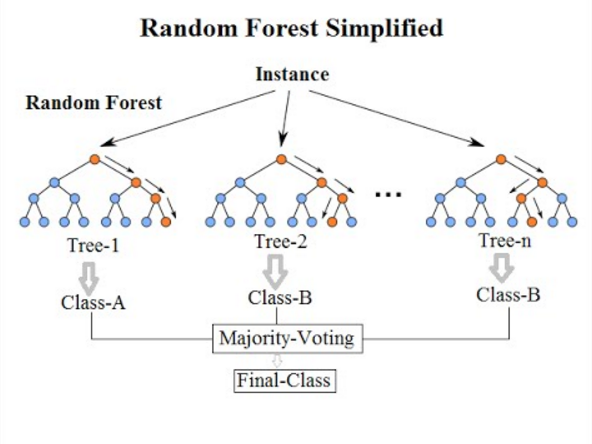
\includegraphics[width=0.6\textwidth]{figures/random-forest.png}
 \caption[test]{Decision process of a Random Forest using majority voting\footnotemark}
 \label{fig:random_forest}
\end{figure}
\footnotetext{Picture taken from https://miro.medium.com/max/1184/1*i0o8mjFfCn-uD79-F1Cqkw.png}



\newpage


\section{Evaluation Metrics}
\label{sec:background evaluation}
The evaluation metric reflects how the model performs. Picking a good evaluation metric is therefore an important step. We will use different evaluation metrics throughout this thesis:

\paragraph{Accuracy.} Accuracy is probably the mostly used and intuitive evaluation metric. It is computed as the total number of correct predicted samples over the total number of samples. It can be computed over all classes or be specific to one class. It gives a taste of what fraction of time we are making good prediction.

\\



 \paragraph{Precision and Recall.} 

Accuracy, is sometime not enough to evaluate a model. To gain more insight, we will also use precision and recall. Before explaining what precision and recall is, we will have to defined the following quantities:

\begin{itemize}
    \item \textbf{True Positive (TP):} Number of samples belonging to a particular class \textbf{correctly} predicted to belong to this class.
    
    \item \textbf{True Negative (TN):} Number of samples \textbf{not} belonging to a particular class \textbf{correctly} predicted to \textbf{not} belong to this class.

    \item \textbf{False Positive (FP):} Number of samples \textbf{not} belonging to a particular class \textbf{wrongly} predicted to belong to this class.

    \item \textbf{False Negative (FN):} Number of samples belonging to a particular class \textbf{wrongly} predicted to \textbf{not} belong to this class.
\end{itemize}

Precision and recall can then be computed with the following formulas:
\begin{itemize}
    \item $Precision=\frac{TP}{TP + FP}$
    \item $Recall = \frac{TP}{TP + FN}$
\end{itemize}

Precision represents the fraction of time we are correct about a class when predicting this class. Whereas recall represents the ability of detecting a certain class when that class appears. These metrics are particularly useful to evaluate the performance of a particular class. We would expect an attacker targeting fitness apps to find the best spot for its advertising campaign, to privilege a good recall score on fitness apps than a good precision score. On the opposite, we would expect an attacker targeting students cheating with their smartwatch to privilege a good precision score. 



\paragraph{F-beta score.} The F-beta score is a mixture of precision and recall. It is computed as the weighted harmonic mean between recall and precision. When the weight beta is equal to 1 we are talking about F1 score which means that we are caring equally much about precision than recall. The F-beta score is computed as follows:


$$ F_\beta = (1 + \beta^2) \cdot \frac{\mathrm{precision} \cdot \mathrm{recall}}{(\beta^2 \cdot \mathrm{precision}) + \mathrm{recall}}$$


\paragraph{Confusion Matrix.} Confusion Matrix are useful representations that assess the performance of a classifier. In our case, each raw of the matrix represents the normalized number of true instances belonging to a particular class while each column represents the predicted instances belonging to a particular class. The diagonal of the matrix represents the normalized number of correct classified predictions.




\paragraph{Cross-validation.}

Cross-validation is a technique used to evaluate a model which provides better confidence about the performance. It consists of splitting train and test data multiple times differently. This ensures that not always the same data are used as train and test. There exists multiple variations of cross-validation. In our case we will use n-Random-Split cross-validation which consists of splitting train and test data randomly n times.